\chapter{実装}
本章では,ADLoggerシステムの実装について述べる.
はじめに実装環境について述べ,ついでタスク別時間記録モジュール,必要時間予測モジュールについて説明する.

\section{実装環境}
本節では,本システムにおける実装環境について説明する.本システムはiPhoneアプリケーションであり,実装言語にはSwiftを使用している.
サーバサイド兼データベースには,MBaaS (Mobile Backend as a Service)であるBack4App~\cite{back4app}を利用している.

\section{クライアント側実装}
クライアントはiPhoneアプリケーションであり,Swiftによって実装した.
タスク別時間記録モジュール,必要時間予測モジュールについて説明する.

\subsection{タスク別時間記録モジュール}
本節ではタスク別時間記録モジュールについて説明する.
タスク別時間記録モジュールはユーザが行動したタスク及び時間を記録するモジュールである.
ログイン後,トップ画面の``TIMER"ボタンを押すと,ストップウォッチ画面に移動する.
``START"ボタンを押すと``START"ボタンは``STOP"ボタンに名前が書き換えられた後,上段の数字`00:00:00"からカウントアップが表示される.
``STOP"ボタンを押すとタスク別時間記録モジュールによって図~\ref{fig:study_alert}のようなUIAlertControllerが表示される.
このUIAlertControllerは,``終了"と``計測に戻る"と``Reset"の3つの選択肢を持っている.

\begin{figure}[ht]
\begin{center}
\begin{tabular}{c}

	\begin{minipage}[b]{0.5\linewidth}
	\begin{center}
		\fbox{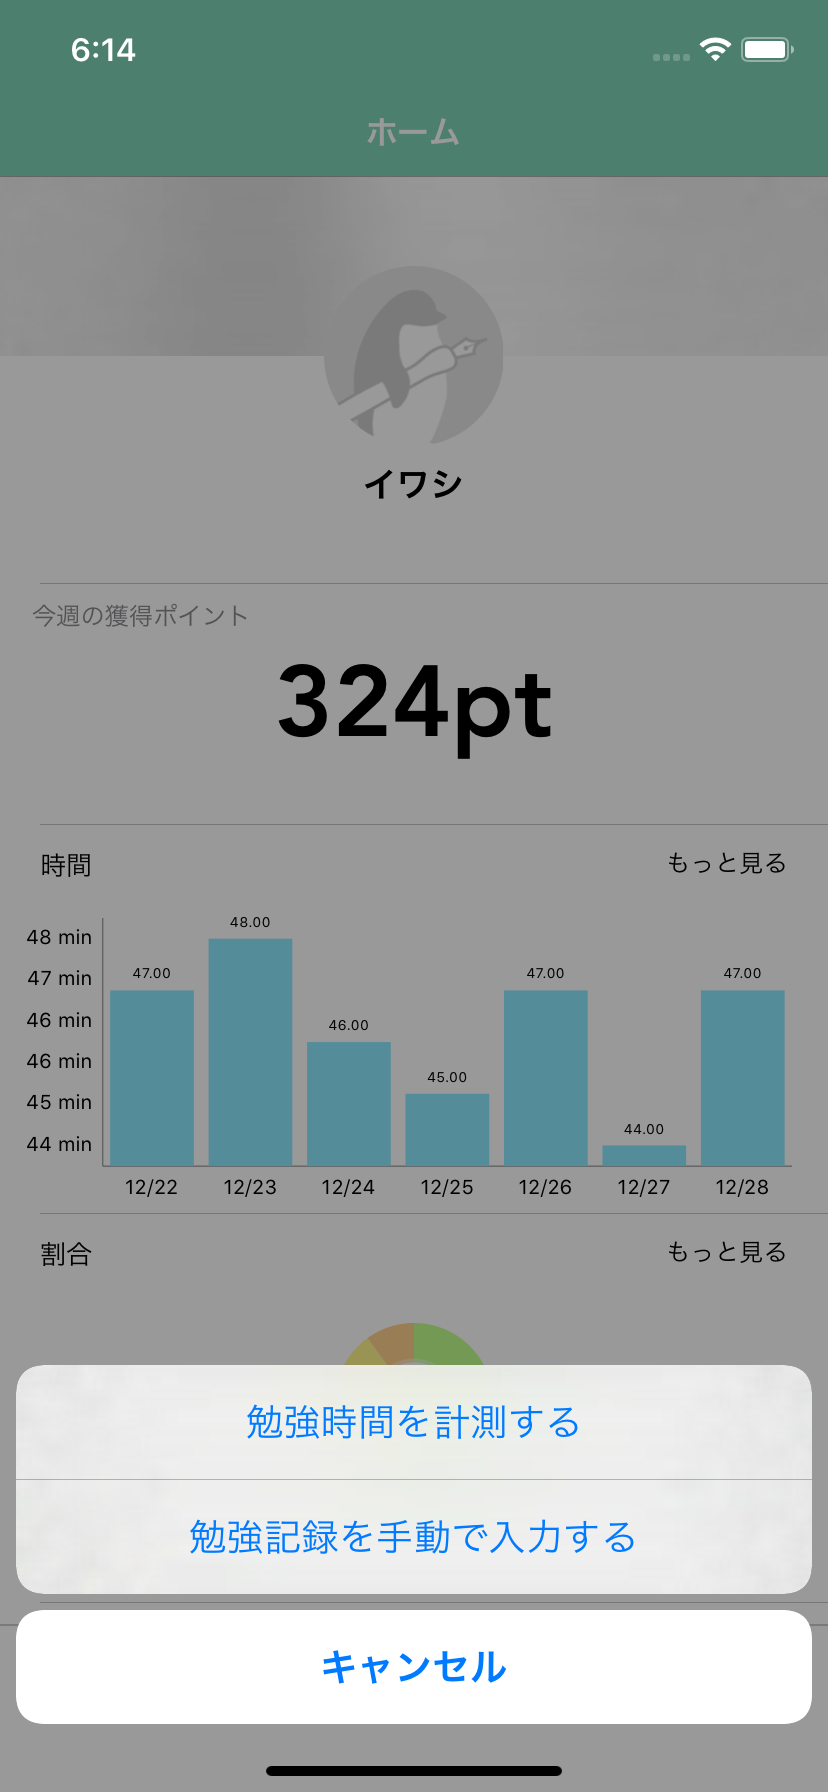
\includegraphics[width=5cm]{images/6/study_alert.png}}
		\caption{記録の仕方を選択させるAction sheet}
		\label{fig:study_alert}
	\end{center}
  	\end{minipage}

  	\begin{minipage}[b]{0.5\linewidth}
	\begin{center}
		\fbox{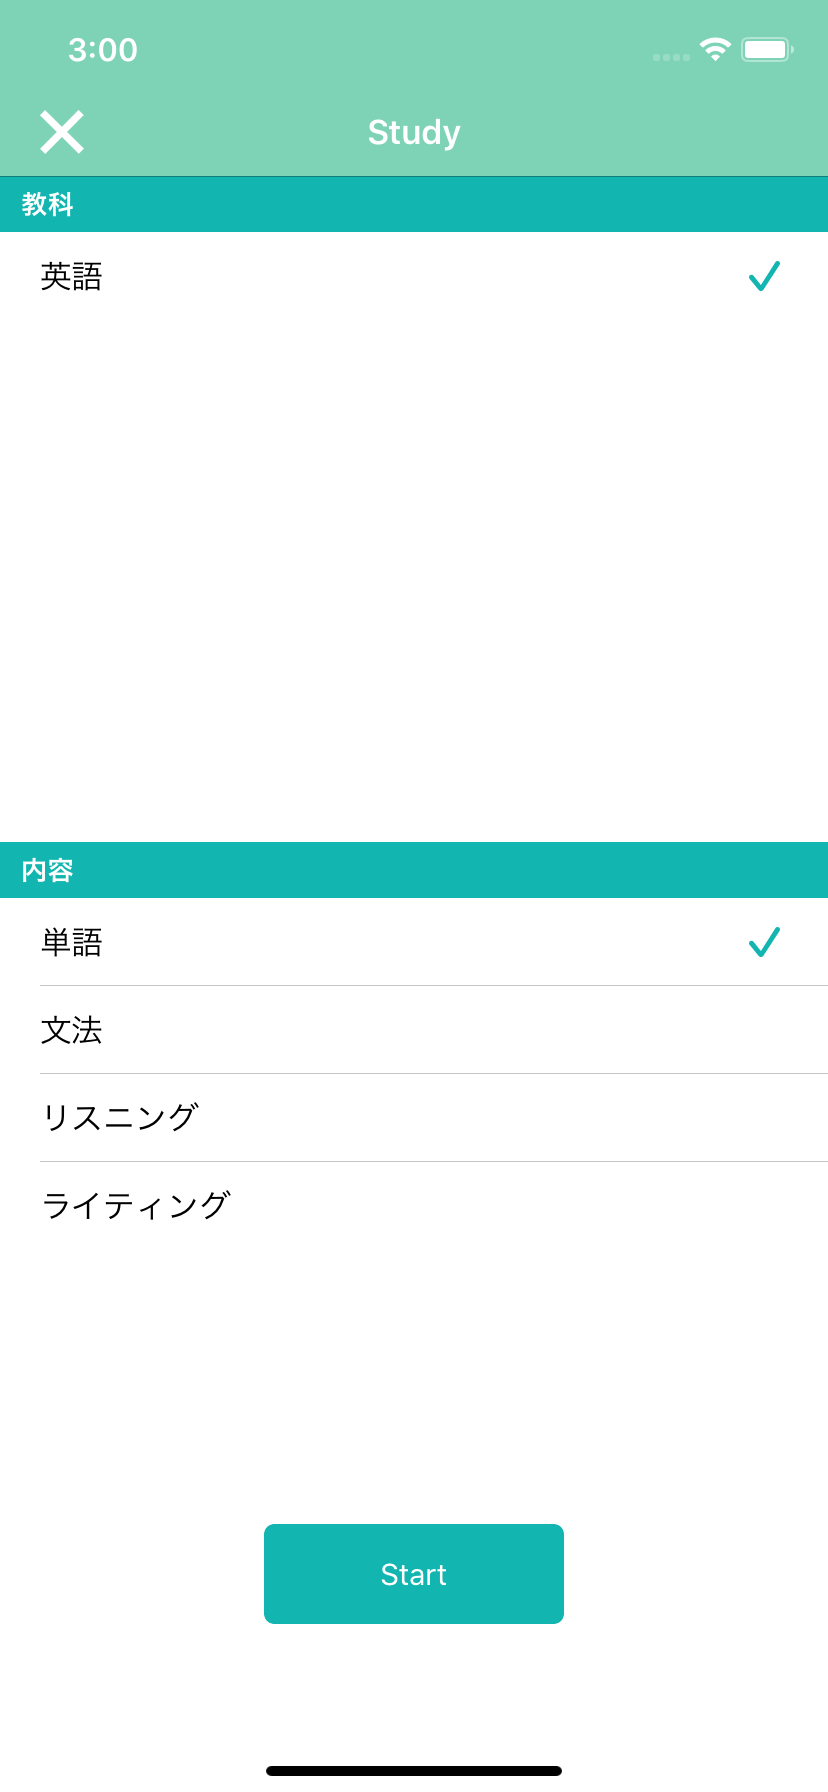
\includegraphics[width=5cm]{images/6/study_select.png}}
		\caption{教科及び内容の選択画面}
		\label{fig:study_select}
	\end{center}
  	\end{minipage}

  	\end{tabular}
  \end{center}
\end{figure}

% ここから後日ちゃんと書く。後上の写真も置き換える!
``計測に戻る"を選択すると,``STOP"ボタンは``START"ボタンに名前が書き換えられた後,カウントアップが再開される.
``Reset"を選択すると,上段の数字はカウントアップを終了し``00:00:00"に書き換えられる事でリセット状態となる.
``終了"を選択するとカウントした数値をInt型で型で渡し,タスク選択画面へ遷移する.
タスク選択画面ではUITableViewで過去記録した事のあるタスク名が表示される.
右上の``新規追加"を押すと
UITableViewCellをタップすると内容を選択することができる.



\subsection{必要時間予測モジュール}
続いて,必要時間予測モジュールについて説明する.
\section{まとめ}
本章では,ADLoggerシステムの実装について述べた.
次章では,本システムで得られたデータから動機づけの向上を評価し,考察について述べる.
